\documentclass[crop,tikz]{standalone}

\usetikzlibrary{
	chains,
	positioning,
	arrows.meta,
	decorations.pathreplacing,
	calc,
	fit,
	shapes.geometric
}

\begin{document}

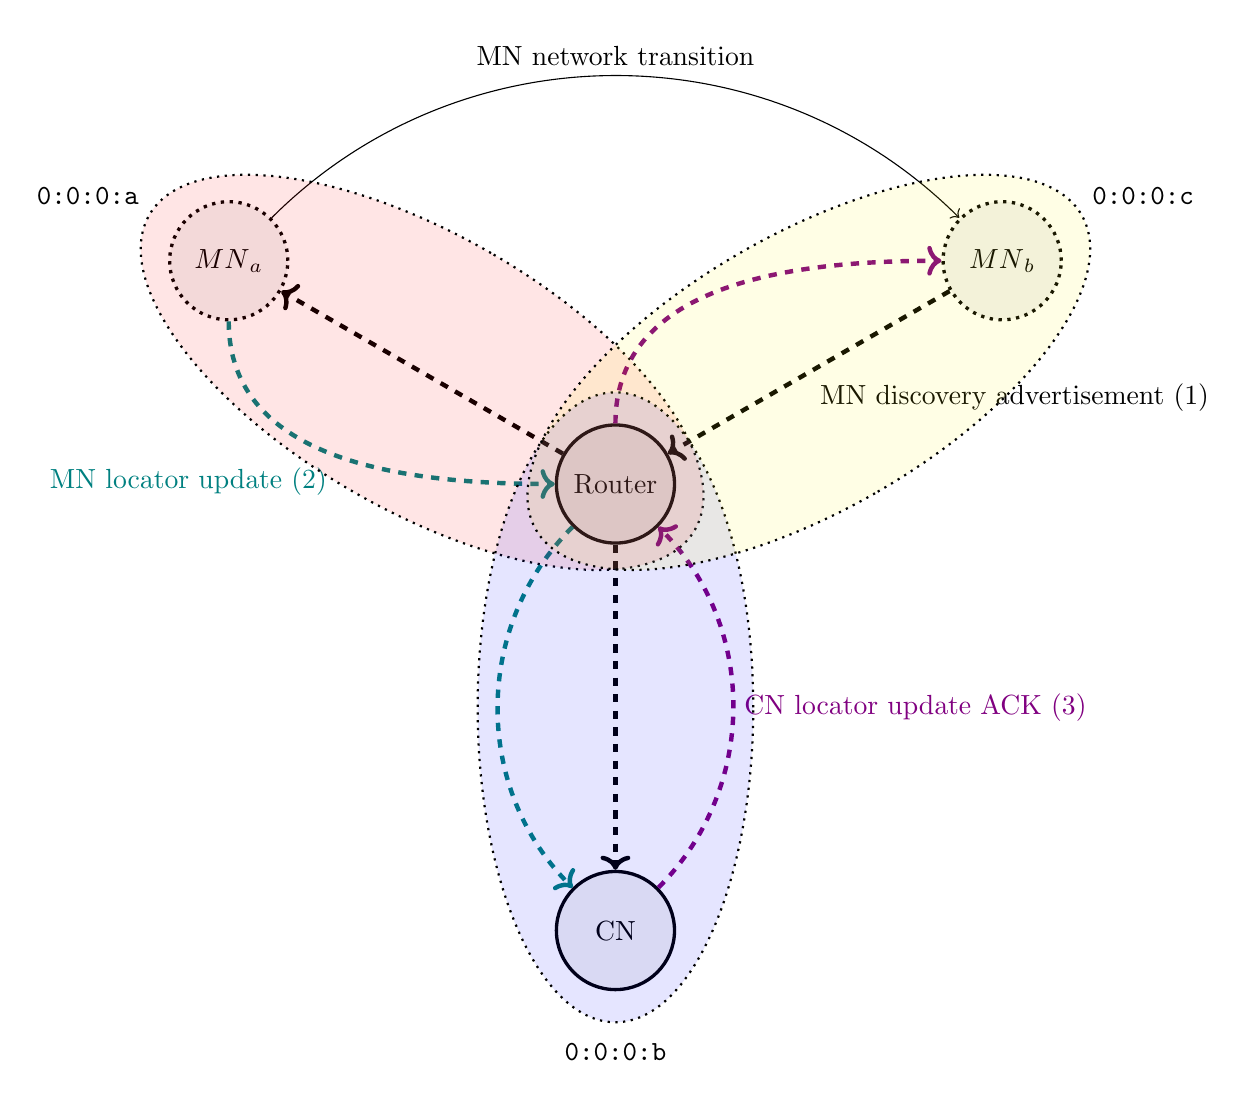
\begin{tikzpicture}[
	nwknode/.style={
		circle,
		very thick,
		minimum size=1.5cm,
		draw,
		fill=black!5,
	},
	network/.style args = {#1}{
		draw,
		ellipse,
		minimum height=8cm,
		minimum width=3.5cm,
		inner xsep=0mm, 
		inner ysep=3mm,
		thick,
		dotted,
		fill=#1,
		fill opacity=0.1,
		text opacity=1,
	}
]
	\node[regular polygon, regular polygon sides=3, inner sep=2cm, rotate=60] (a) {};
	\node[regular polygon, regular polygon sides=3, inner sep=2cm] (c) {};
	
	\node[nwknode] (r) at (a) {Router};
	\node[nwknode] (cn)  at (a.corner 2) {CN};
	\node[nwknode, dotted] (mn_a)  at (a.corner 1) {$\text{MN}_a$};
	\node[nwknode, dotted] (mn_b)  at (a.corner 3) {$\text{MN}_b$};
	
	\draw[->] (mn_a) to[out=45,in=135] node[above] {MN network transition} (mn_b);
	
	\draw[ultra thick,dashed,->] (mn_b) -- node[below right] {MN discovery advertisement (1)} (r);
	\draw[ultra thick,dashed,->] (r) -- node[right] {} (cn);
	\draw[ultra thick,dashed,->] (r) -- node[right] {} (mn_a);
	
	\draw[ultra thick,dashed,teal,->] (mn_a) to[out=-90,in=180] node[below left] {MN locator update (2)} (r);
	\draw[ultra thick,dashed,teal,->] (r) to[out=-135,in=135] node[left] {} (cn);
	
	\draw[ultra thick,dashed,violet,->] (cn) to[out=45,in=-45] node[right] {CN locator update ACK (3)} (r);
	\draw[ultra thick,dashed,violet,->] (r) to[out=90,in=180] node[below right] {} (mn_b);
	
	% horribly hacky
	\node[network={red}, rotate=60, label=\texttt{0:0:0:a}] at (c.side 1) {};
	\node[network={blue}, rotate=0, label={[anchor=south,above=-6mm]270:\texttt{0:0:0:b}}] at (c.side 2) {};
	\node[network={yellow}, rotate=-60, label=\texttt{0:0:0:c}] at (c.side 3) {};
\end{tikzpicture}

\end{document}